\documentclass[12pt,compress]{beamer}
%\documentclass[handout,t]{beamer}

\batchmode
% \usepackage{pgfpages}
% \pgfpagesuselayout{4 on 1}[letterpaper,landscape,border shrink=5mm]

\usepackage{amsmath,amssymb,enumerate,epsfig,bbm,calc,color,ifthen,capt-of,multicol}

\usepackage[all,pdf]{xy}

% add page number
\expandafter\def\expandafter\insertshorttitle\expandafter{%
	\insertshorttitle\hfill%
	\insertframenumber\,/\,\inserttotalframenumber}

\usetheme{Berlin}
\usecolortheme{umji}

\title{Thermodynamics in VC210}
\author{Haotian Fu}
\institute{University of Michigan--Shanghai Jiao Tong University Joint Institute}
\date{\today}
\pgfdeclareimage[height=0.5cm]{umji-logo}{umji.pdf}

\logo{\pgfuseimage{umji-logo}\hspace*{0.5cm}}

\AtBeginSection[]
{
  \begin{frame}<beamer>
    \frametitle{Outline}
    \tableofcontents[currentsection]
  \end{frame}
}
\beamerdefaultoverlayspecification{<+->}

% -----------------------------------------------------------------------------
\begin{document}

% -----------------------------------------------------------------------------

\lecture{RC_3}

\frame{\titlepage}

\section[Outline]{}
\begin{frame}{Outline}
    \tableofcontents
\end{frame}

% -----------------------------------------------------------------------------

\section{Concept Review}
\subsection{1$^{st}$ Law}
\begin{frame}{First law of thermodynamics}
    \begin{equation}
        U = Q + W
    \end{equation}
    \textbf{Remarks:}
    \begin{itemize}
        \item Differential form \& $U = f\,(T)$
        \item $W$ - work, including expansion work and non-expansion work. However, we only discuss the expansion work here.
        \item $Q$ - heat, can be modelized as $Q_V$ and $Q_p$
    \end{itemize}
\end{frame}
\begin{frame}{Enthalpy}
    \begin{equation}
        H = U + pV
    \end{equation}
    \textbf{Remarks:}
    \begin{itemize}
        \item Differential form \& $H = f\,(T)$.
        \item Pay attention to the common name of enthalpys, such as, $H_{vap}$, $H_{fus}$, $H_{sub}$.
        \item $pV$ should be fully understood.
    \end{itemize}
\end{frame}
\begin{frame}{Heat capacity}
    \begin{equation}
        C = \lim\limits_{\Delta T \rightarrow 0}\frac{\Delta Q}{\Delta T}
    \end{equation}
    \textbf{Remarks:}
    \begin{itemize}
        \item Heat capacity \& specific heat capacity.
        \item $Q$ should be fully understood.
        \item Relationship with Kinetic Molcular Theory (KMT).
    \end{itemize}
\end{frame}
\begin{frame}{KMT \& Heat capacity\footnote{\tiny{You may refer to \textit{Chemicle Principle} pp. 402}}}
    \begin{figure}[H]
        \centering
        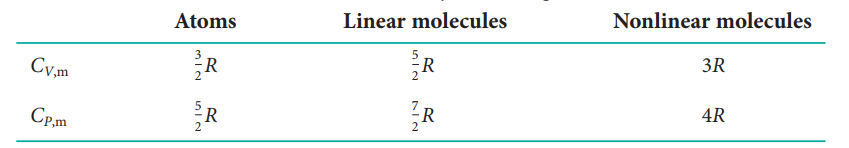
\includegraphics[width=\textwidth]{KMT.png}
        \caption{$C_{V,m}$ and $C_{p,m}$ of three types of molecules.}
    \end{figure}
\end{frame}

\subsection{2$^{nd}$ Law}
\begin{frame}{The second law of thermodynamics}
    \begin{block}{Clausius Statement}
        Heat can never pass from a colder to a warmer body without some other change, connected therewith, occurring at the same time.
    \end{block}
\end{frame}
\begin{frame}{The second law of thermodynamics}
    \begin{block}{Kelvin Statement}
        It is impossible for a self-acting machine, unaided by any external agency, to convey heat from one body to another at a higher temperature. \\
        It is impossible, by means of inanimate material agency, to derive mechanical effect from any portion of matter by cooling it below the temperature of the coldest of the surrounding objects.
    \end{block}
\end{frame}
\begin{frame}{Entropy}
    \begin{equation}
        dS = \frac{\delta Q_R}{T}
    \end{equation}
    \textbf{Remarks:}
    \begin{itemize}
        \item The intuition of entropy.
        \item Entropy criterion.
        \item Calculation of entropy.
    \end{itemize}
\end{frame}
\begin{frame}{Gibb's Free Energy}
    \begin{equation}
        G = H - TS
    \end{equation}
    \begin{itemize}
        \item Differential form.
        \item Comparing with $\Delta G = \Delta H - T \Delta S$
        \item Gibb's free energy criterion.
        \item Calculation of Gibb's free energy.
    \end{itemize}
\end{frame}


\subsection{3$^{rd}$ Law}
\begin{frame}{The third law of thermodynamics}
    $$
        S \rightarrow c\quad \text{as}\quad T \rightarrow 0\,\text{K}
    $$
    Especially, $c=0$ when the object is \textbf{perfect crystal}.
\end{frame}

\subsection{0$^{th}$ Law}
\begin{frame}{The zeroth law of thermodynamics}
    \begin{block}{content}
        If two thermodynamic systems are each in thermal equilibrium with a third system, then they are in thermal equilibrium with each other.
    \end{block}
\end{frame}

\subsection{Practical Formula}
\begin{frame}{Practical Formula}
    \begin{align}
         & Q_V = \Delta U                                      \\
         & Q_p = \Delta H                                      \\
         & C_V = \frac{\Delta U}{\Delta T}                     \\
         & C_p = \frac{\Delta H}{\Delta T}                     \\
         & \Delta S_{\text{surrounding}} = -\frac{\Delta H}{T} \\
         & S=k\ln W
    \end{align}
\end{frame}
\begin{frame}{Practical Formula}
    \begin{align}
         & \text{phase change } \nonumber                                                         \\
         & \Delta S = \frac{Q_R}{T}                                                               \\
         & \text{physical change with constant pressure } \nonumber                               \\
         & \Delta S = nC_{V,m}\ln\left(\frac{T_2}{T_1}\right) + nR\ln\left(\frac{V_2}{V_1}\right) \\
         & \text{physical change with constant volume } \nonumber                                 \\
         & \Delta S = nC_{p,m}\ln\left(\frac{T_2}{T_1}\right) + nR\ln\left(\frac{p_1}{p_2}\right)
    \end{align}
\end{frame}
\begin{frame}{Practical Formula}
    \begin{align}
         & \text{Clausius–Clapeyron relation} \nonumber                                                  \\
         & \ln\left(\frac{p_2}{p_1}\right) = -\frac{\Delta H}{R}\left(\frac{1}{T_2}-\frac{1}{T_1}\right) \\
         & \text{constant temperature} \nonumber                                                         \\
         & \Delta G = \int V dp \quad \text{since}\quad dG = -sdT + Vdp
    \end{align}
\end{frame}

% -----------------------------------------------------------------------------

\section{Examples}
\begin{frame}{Bohn-Haber Cycle}
    \begin{block}{}
        The standard molar enthalpy of combustion of ethanol (C$_2$H$_5$OH) and acetic acid (CH$_3$COOH) is -136.50 and -67.50 kJ/mol. \\
        The enthalpy of dissolution is 11.71 and 1.46 kJ/mol correspondingly. Calculate the enthalpy of oxidation of thtanol in water solution.
    \end{block}
\end{frame}
\begin{frame}{Liquid-Solution}
    \begin{block}{}
        Liquid $A$ and $B$ form an ideal solution. The solution containing 1 mol $A$ and 2 mol $B$ at 343.2 K has a vapor pressure of 50.663 kPa. \\
        If 3 mol $A$ is added, the vapor pressure of the solution increases to 70.928 kPa. Calculate (1) $p_A^*$ and $p_B^*$ at 343.2 K; (2) the gaseous composition of the first mixed solution.
    \end{block}
\end{frame}



%------------------------------------------------------------------------------

\end{document}